% Chapter 3

\chapter{The Bayesian approach: Hierarchical Bayesian modeling}
\label{chapter:bayesian}


%----------Intro - general concepts --------------------------------------------------------
\section{Introduction - General concepts}
\label{sec:bayes_intro}
%%%%%%%%%%%%%%%%%%%%%%%%%%%%%%%%%%%%%%%%%%%%%%%%%%%%%%%%%%%%%%%%%%%%%%%%%%%%%%%

Over the last two decades, sparsity has emerged as a key concept to solve inverse problems such as tomographic image reconstruction, deconvolution or inpainting, but also to regularize high dimensional regression problems in the field of machine learning. There are mainly two routes to introduce sparsity to such problems.\\

The first route, embraced by the optimization community and frequentist
statisticians, is to promote sparsity using convex optimization theory.
This line of work has led to now mature theoretical guarantees~\cite{FoRa13} when using regularization functions based on $\ell_1$ norm and other convex variants~\cite{Tibshirani96}. In particular, it has been popularized in the signal processing community under the name of compressed sensing~\cite{candes2008introduction} when combined with incoherent measurements.

There are however some limitations of sparsity promoting convex penalties based
on the $\ell_1$ norm.
All the features (also called regressors, atoms or sources depending
on the terminology of the community) involved
in the solution form what is called the support of the solution.
Convex penalties can fail to identify the correct support in the presence of highly noisy data, but also in low noise setups if the forward operator (referred to as design matrix in statistics) is poorly conditioned.
Convex regularizations also leads to a systematic underestimation bias
in the amplitude of the coefficients~\cite{OsBuGoXuYi06,Candes,chartrand2007exact,saab2008stable,ChHeSa17}.

To address these limitations of $\ell_1$-type models,
reweighted schemes have been
proposed~\cite{Candes,Gasso,Rakotomamonjy,zhang-rao:2011,strohmeier-etal:16}, of which the Adaptive Lasso~\cite{Zou06} is the most commonly used in the statistics community:
Starting from the Lasso estimator, which amounts to regressing with a standard $\ell_1$-norm as a regularizer (this estimator is sometimes referred to as Basis Pursuit Denoising (BPDN)~\cite{Chen_Donoho_Saunders98} in signal processing), the Adaptive Lasso solves a sequence of weighted Lasso problems, where at each iteration the
weights are chosen such that the strongest coefficients are less and less penalized.
From the optimization point of view, such an iterative scheme can be derived from so-called majorization-minimization (MM) strategies~\cite{lange2000optimization,schifano2010majorization}.
The idea behind MM is to minimize the objective function by successively minimizing upper bounds that are easier to optimize. Many well-known optimization approaches can be interpreted as instances of MM, \eg simple gradient descent or proximal algorithms~\cite{Combettes2011}, expectation-maximization (EM)~\cite{Dempster77maximumlikelihood}, and difference-of-convex (DC) programming techniques~\cite{Horst:1999}.
%
More recently, re-weighted $\ell_1$-norm schemes based on MM principle have been particularly popular to handle concave, hence non-convex regularizations such as $\ell_{1/2}$-quasi-norms or logarithmic functions. As such, these schemes are prone to converging to a local minimum determined by the initial, uniformly weighted $\ell_1$-norm solution (\ie the Lasso estimator) that constitutes the first iterate.\\

The second route to introduce sparsity formulates the regression problem in a Bayesian framework and uses hierarchical Bayesian models (HBM) \cite{mackay2003information} for the inference.
The common way to formulate HBMs is to consider the variance parameters of Gaussian prior models as additional random variables which have to be estimated from the data as well. Their prior distributions are referred to as hyper-priors. Plausible solutions to the regression problem that both fit data and the \emph{a priori} assumption of sparsity are explicitly characterized as multiple distinct modes of the posterior distribution. This characterization is the Bayesian analogue to local minima in variational regression approaches when working with non-convex functionals. Different strategies to infer a point estimate for the parameters of interest from the \emph{a posteriori} distribution then lead to different algorithmic frameworks, for instance Variational Bayesian approaches~\cite{mackay2003information,jordan1999introduction,sato2004hierarchical,FrHaDaKiPhTrHeFlMa08,shervashidze2015learning}, Sparse Bayesian Learning (SBL) approaches (also referred to as type-I or type-II maximum likelihood estimates) \cite{tipping2001sparse,wipf2004sparse,Wipf-Nagarajan:2009,zhang-rao:2011} and fully-Bayesian strategies \cite{CaHaPuSo09,Lucka-etal:2012}.
In this work, we focus on the later one for a non-standard type of HBM examined in \cite{Lu14} that combines a non-Gaussian prior with an $\ell_{1}$-type energy function with a specific Gamma hyper-prior.
For this HBM, a simple alternating scheme to compute full maximum \emph{a posteriori} (MAP) estimates leads to exactly the same sequence of problems solved by MM applied to $\ell_{1/2}$-type regularizations.
With this observation made, it is natural to revisit and improve these MM schemes by leveraging the ability of the Bayesian framework to explore the modes of the posterior distribution by Markov chain Monte-Carlo (MCMC) schemes \cite{RoCa05,KaSo05}. This can not only mitigate the aforementioned initialization-dependence of MM, but more importantly, it offers insights into the structure and importance of potentially multiple plausible sparse solutions. Yet, the benefit comes at the cost of additional computational efforts.

Magnetoencephalography (MEG) and electroencephalography (EEG) are technologies that allow to measure the electromagnetic fields produced by active neurons in a non-invasive way. Localization of foci of neural activations from MEG/EEG recordings is a high impact problem both for cognitive neuroscience and clinical neuroscience, with applications in pathologies such as epilepsy, sleep research or neurodegenerative disorders. Despite the linearity of the forward problem, this inverse problem is
particularly challenging as the forward operator is both under-determined and strongly
ill-conditioned.
As such, both non-convex optimization strategies with reweighted schemes~\cite{strohmeier-etal:16} and hierarchical Bayesian approaches have been proposed~\cite{sato2004hierarchical,CaHaPuSo09,Wipf-Nagarajan:2009,Sorrentino-etal:2009,Lucka-etal:2012} for M/EEG source localization. For this reason, it is an ideal application for our examinations.\\

The manuscript is organized as follows: First, we present in a unified
perspective on both routes to sparsity, \ie reweighted $\ell_1$ MM schemes
and specific HBMs. We show that a particular, optimization based inference strategy recovers the MM algorithm. We then describe an HBM inference strategy based upon an MCMC sampling and show on simulated and experimental M/EEG datasets how these stochastic MCMC-based techniques can not only help to improve upon deterministic approaches but also help to reveal multiple plausible solutions to the inverse problem. This analysis leads to an uncertainty quantification (UQ) of the support recovery of non-convex sparse regression problems that provides very useful complementary information, in particular for very ill-conditioned and under-determined applications like M/EEG source localization.

%----------Lp hypermodels ------------------------------------------------------------------
\section{Lp hyper-models}

%----------MAP estimation ------------------------------------------------------------------
\section{MAP estimation}

%----------Link between MM & HBM------------------------------------------------------------
\section{Link between MM and special case of HBM}
(Comparison \& Equivalence)
We start this section by recalling how majorization-minimization works
when addressing variational formulations with concave, hence non-convex, regularization.
It is followed by an introduction to hierarchical Bayesian models with Gamma hyper-priors.
Then, we explain how these seemingly different approaches can lead to the
exact same regression algorithm.
From this, we detail how different Bayesian inference strategies using MCMC
sampling can more precisely explore the landscape of the posterior distribution of the HBM model and provide multiple possible solutions to the sparse regression problem compared to MM.

\subsection{MM}
\label{sub:MM}

Majorization-Minimization (MM) strategies consist in replacing a difficult
optimization problem with a series of easier ones that are obtained by
upper bounding the objective function, often by a convex majorant.
%
In the context of inverse problems or high-dimensional statistics using sparsity constraints,
MM has been successfully applied to address non-convex regularization terms.
An example is the regression model with $\ell_{2,p}$-quasi-norms regularization
over the groups when $0<p<1$: The desired estimate $\hat{\bfX}$ is defined as one of potentially multiple minimizers of
\begin{equation} \label{eq:L2pReg}
\hat{\bfX} \in \argmin_{\bfX\in\R^{q \times t}} \frac{1}{2} \fronormsq{\bfM - \bfG \bfX}  + \lambda \sum_{i=1}^n \fronorm{\bfX_{[i]}}^p \enspace,
\end{equation}
where $\lambda > 0$ is the regularization parameter balancing the data fit and the penalty term. One possible MM approach to solve Eq.\textbf{XXX-eref{eq:L2pReg}} %~\eref{eq:L2pReg}
with $p=1/2$ would consist of minimizing a sequence of non-smooth convex surrogate functions where the non-convex regularization is replaced by a weighted $\ell_{2,1}$ norm~\cite{strohmeier-etal:16}. In each iteration, the weights are derived from the current estimate of $\bfX$.

Due to the concavity of the non-decreasing function $\bfX\mapsto\sqrt{\fronorm{\bfX}}$, it is upper bounded by its tangent and a first order Taylor expansion at the current estimate $\bfX_{[i]}$ provides an upper bound that can be used to construct the non-smooth convex surrogate problem. By solving this sequence of surrogate problems, the value of the non-convex objective function is guaranteed to decrease. However, due to the non-convexity, only convergence towards a local minimum can be guaranteed.


For the problem in Eq.\textbf{XXX-eref{eq:L2pReg}} %~\eref{eq:L2pReg}
 with $p=1/2$, the $k^{th}$ iteration of the MM scheme reads:
\begin{eqnarray}
\label{eq:MM}
\fl \quad \hat{\bfX}^{(k)} \in \argmin_{\bfX\in\R^{q \times t}} \frac{1}{2} \fronormsq{\bfM - \bfG \bfX}  + \lambda \sum_{i=1}^n \frac{ \fronorm{\bfX_{[i]}} }{ \bfw^{(k-1)}_{i}}, \qquad \bfw^{(k-1)}_{i} = 2 \sqrt{\fronorm{\bfX^{(k-1)}_{[i]}}} \enspace.
\end{eqnarray}
As each weight $\bfw^{(k)}_{i}$ is a non-decreasing function of $\fronorm{\bfX^{(k)}_{[i]}}$, sources with high amplitudes in one iteration will be less penalized in the next iteration and can better explain the data $\bfM$. Sources for which $\fronorm{\bfX^{(k)}_{[i]}} = 0$ at a certain iteration $k$ are effectively pruned from the model for all following iterations. Using MM therefore leads to a solution that explains the data with fewer active  locations $i$ compared to a standard $\ell_{2,1}$ norm regularized solution.
Note that a default initialization consists in setting $\bfw^{(0)}_{i}=1, \forall i \in [n]$.

To exploit existing fast solvers for the $\ell_{2,1}$ regularized problems~\cite{strohmeier-etal:16,Ndiaye_Fercoq_Gramfort_Salmon15}, we reformulate the weighted subproblem and apply the weights by scaling the matrix $\bfG$ with a diagonal matrix $\bfW^{(k)} \in \bbR^{dn \times dn}$ given by:
\begin{eqnarray} \label{eq:weights}
\bfW^{(k)} = \mathrm{diag}(\bfw^{(k)} \otimes \mathbf{1}_{d}) \enspace ,
\end{eqnarray}
where $\bfw^{(k)} \in \bbR^{n}$, $\mathbf{1}_{d}\in\R^d$ is a vector of ones and $\otimes$ is the Kronecker product.
Defining $\tilde{\bfG}^{(k)}=\bfG \bfW^{(k-1)}$, the reformulated problem reads:
\begin{eqnarray}\label{eq:lasso_new_gram}
\tilde{\bfX}^{(k)} &
% = \argmin_{\bfX\in\R^{q \times t}} \frac{1}{2}\fronormsq{\bfM - \bfG \bfW^{(k)}\bfX}  + \lambda \sum_{i=1}^n \fronorm{\bfX_{[i]}} \\
 & \in \argmin_{\bfX\in\R^{q \times t}} \frac{1}{2}\fronormsq{\bfM - \tilde{\bfG}^{(k)} \bfX}  + \lambda \sum_{i=1}^n \fronorm{\bfX_{[i]}} \enspace .
\end{eqnarray}
After convergence, we reapply the scaling to $\tilde{\bfX}$ to obtain $\hat{\bfX}$:
\begin{equation}
    \label{eq:MM_weights}
    \hat{\bfX}^{(k)} = \bfW^{(k-1)} \tilde{\bfX}^{(k)} \enspace .
\end{equation}
The reformulation through Eq.\textbf{XXX} %Eq.~\eref{eq:lasso_new_gram}
 and Eq.\textbf{XXX} % \eref{eq:MM_weights}
 avoids any division by zero when $\bfX^{(k-1)}=0$. The above procedure, which matches the strategy of the Adaptive Lasso estimator~\cite{Zou06}, is expressed as pseudo-code in Algorithm~\ref{alg:adpative_lasso}. More technical details can be found in~\cite[Algorithm 3]{strohmeier-etal:16}.


{\fontsize{4}{4}\selectfont
%above is to make smaller fonts in algorithm
\begin{algorithm}[t]
\SetKwInOut{Input}{input}
\SetKwInOut{Init}{init}
\SetKwInOut{Parameter}{param}
\caption{\textsc{$\ell_{2,p}$ MM algorithm with $p=1/2$ (Adaptive Lasso)}}
\Input{$\bfM, \bfG,\lambda > 0, \bfW^{(0)} \geqslant 0,\epsilon > 0, \tau > 0$ and $K$ }
% \Parameter{ To add }
%\Init{$\bfW^{(1)}=I_{dn\times dn}$ }
\For{
        $k = 1$ to $K$
    }
    {
		$\tilde{\bfG}^{(k)} = \bfG \bfW^{(k-1)}$

		Get $\tilde{\bfX}^{(k)}$ solving Eq.\textbf{XXX} at $\epsilon$-precision (e.g. by block coordinate descent).  %~\eref{eq:lasso_new_gram}

		Update $\hat{\bfX}^{(k)} = \bfW^{(k-1)} \tilde{\bfX}^{(k)}$

	    Update $\bfW^{(k)}=\mathrm{diag}(\bfw^{(k)} \otimes \mathbf{1}_{d})$ where $\bfw^{(k)}_{[i]} = 2 \sqrt{\fronorm{\hat{\bfX}^{(k)}_{[i]}}}$,  $\forall i\in [n]$

		\If{ $\norm{\hat{\bfX}^{(k)}-\hat{\bfX}^{(k-1)}}_{\infty} \leq \tau$}{Break}

     }
%\Return{$\hat{\bfX}^{(k)}$}
%\label{alg:adpative_lasso}
\end{algorithm}
}

%%%%%%%%%%%%%%%%%%%%%%%%%%%%%%%%%%%%%%%%%%%%%%%%%%%%%%%%%%%%%%%%%%%%%%%%%%%%%%%
\subsection{Hierarchical Bayesian Modeling}
\label{sub:HBM}
%%%%%%%%%%%%%%%%%%%%%%%%%%%%%%%%%%%%%%%%%%%%%%%%%%%%%%%%%%%%%%%%%%%%%%%%%%%%%%%

In this section, we formulate the inference problem given by Eq.\textbf{XXX:eref}%~\eref{eq:FwdEq}
 and the regularization strategy with $\ell_{2,p}$-quasi-norms from a Bayesian perspective \cite{KaSo05,Lu14}: The Bayesian approach incorporates prior beliefs about the model parameters in terms of probability distributions. Under the AWGN assumption the likelihood of the model is given by:
\begin{eqnarray} \label{eq:like}
\like &\propto \exp \left( - \frac{1}{2} \fronormsq{\bfM - \bfG \bfX} \right) \enspace.
\end{eqnarray}
From Eq.\textbf{XXX:eref}%~\eref{eq:L2pReg}
 we can construct the $\ell_{2,p}$ group prior as:
 \begin{equation} \label{eq:prior}
\prior \propto \exp \left( - \lambda \sum_{i=1}^n \fronorm{\bfX_{[i]}}^p \right)
= \prod_{i=1}^n \exp \left( - \lambda \fronorm{\bfX_{[i]}}^p \right) \enspace,
\end{equation}
which leads to the following posterior probability density using the Bayes rule:
\begin{equation} \label{eq:post}
\post \propto \exp \left( - \frac{1}{2} \fronormsq{\bfM - \bfG \bfX} - \lambda \sum_{i=1}^n \fronorm{\bfX_{[i]}}^p \right) \enspace.
\end{equation}
To extend Eq.\textbf{XXX:eref}%~\eref{eq:prior}
 to a hierarchical prior model \cite{mackay2003information}, we replace the scalar $\lambda$ by a vector of hyper-parameters $\gamma \in \R^{n}_+$ and for any $p \geq 1$ we write the \emph{conditional $\ell_{2,p}$ prior} as:
\begin{equation} \label{eq:condprior}
\fl \hiprior
% \propto \prod_{i=1}^n N(\gamma_i) \exp \left( - \frac{\fronorm{\bfX_{[i]}}^p}{\gamma_i} \right)
\propto \exp \left( - \sum_{i=1}^n \left( \frac{\fronorm{\bfX_{[i]}}^p}{\gamma_i} + \frac{d t}{p} \log(\gamma_i)\right)\right) \enspace,
\end{equation}

where the logarithmic term accounts for the terms of the normalization that depend on $\gamma$ \cite{Lu14}. A common choice for a hyper-prior on each $\gamma_i$ is given by a \emph{Gamma distribution} \cite{mackay2003information,KaSo05,CaHaPuSo09,Lucka-etal:2012} with shape and scale parameters $\alpha$ and $\beta$:
\begin{equation} \label{eq:hyper}
\fl \hyper \propto
\prod_{i=1}^n \gamma_i^{\alpha - 1}
\exp \left(- \frac{\gamma_i}{\beta} \right)
=\exp \left( - \sum_{i=1}^n \left( - \frac{\gamma_i}{\beta} + (\alpha - 1) \log(\gamma_i) \right) \right) \enspace.
\end{equation}
Then, the full posterior over both $\bfX$ and $\gamma$ becomes:
\begin{eqnarray}
\label{eq:full-post}
\fl \hipost \propto \nonumber \\
\fl \hspace{3em} \exp \left( - \frac{1}{2} \fronormsq{\bfM - \bfG \bfX} - \sum_{i=1}^n \left( \frac{\fronorm{\bfX_{[i]}}^p}{\gamma_i} + \frac{\gamma_i}{\beta} - (\alpha - 1 - \frac{dt}{p}) \log(\gamma_i) \right) \right)\enspace.
\end{eqnarray}
The question of how to best derive parameter estimates, in particular how to treat the two different types of parameters $\bfX$ and $\gamma$, distinguishes different HBM-based inference strategies. Variational Bayesian Variational Bayesian approaches ~\cite{mackay2003information,jordan1999introduction,sato2004hierarchical,FrHaDaKiPhTrHeFlMa08,shervashidze2015learning} and Sparse Bayesian Learning \cite{tipping2001sparse,wipf2004sparse,Wipf-Nagarajan:2009,zhang-rao:2011} approaches rely on approximating or marginalizing the full, joint posterior distribution \textbf{XXX:eref}%\eref{eq:full-post}
. In contrast, fully-Bayesian strategies \cite{CaHaPuSo09,Lucka-etal:2012} work with it directly. The most popular one is the full maximum-a-posteriori (\emph{full-MAP}) estimate which is defined as
\begin{eqnarray}
(\xMAP,\gamMAP) & \in \argmax_{(\bfX,\gamma) \in\R^{q \times t} \times \R^{n}_+} \left\lbrace \hipost \right\rbrace \enspace.%,\\
\end{eqnarray}
A common strategy  to compute it is to minimize the \emph{negative log posterior} $-\log \hipost$ by alternating  minimization over $\bfX$ and $\gamma$ (known as \emph{block coordinate descent} in optimization):
\begin{eqnarray}
\label{eq:AO}
\fl \qquad  \bfX^{(k)}& \in \argmin_{\bfX\in\R^{q \times t}} \left\lbrace \frac{1}{2} \fronormsq{\bfM - \bfG \bfX} + \sum_{i=1}^n  \frac{\fronorm{\bfX_{[i]}}^p}{\gamma^{(k-1)}_i} \right\rbrace \label{eq:AO-X}\enspace, \\
\fl \qquad \gamma^{(k)}_i & \in \argmin_{\gamma_i\in \R_+} \left\lbrace\frac{\fronorm{\bfX^{(k)}_{[i]}}^p }{\gamma_i} + \frac{\gamma_i}{\beta} - (\alpha - 1 - \frac{dt}{p}) \log(\gamma_i) \right\rbrace, \quad \forall i\in [n] \enspace. \label{eq:AO-gamma}
\end{eqnarray}
Other fully-Bayesian estimates are defined as integrals of functions of $\bfX$ and $\gamma$ with respect to the posterior distribution, \eg first or second moment estimates. To compute these high dimensional integrals efficiently, only Markov chain Monte-Carlo (MCMC) methods that draw correlated samples from the posterior distribution can be used\cite{RoCa05,KaSo05} . A commonly used MCMC scheme for HBM is given by \emph{blocked Gibbs sampling} which alternates as:
\begin{eqnarray}
\bfX^{(k)} &\sim \: p_{post}(\bfX,\gamma^{(k-1)}|\bfM) &\propto p_{post}(\bfX|\bfM,\gamma^{(k-1)}) \enspace, \label{eq:AS-X}\\
\gamma^{(k)} &\sim \: p_{post}(\bfX^{(k)},\gamma|\bfM) &\propto p_{post}(\gamma|\bfM,\bfX^{(k)})\enspace. \label{eq:AS-gamma}
\end{eqnarray}
In this study, however, we are not interested in sampling the posterior distribution for computing the integral-based estimators but we rather want to explore the different modes of this multi-modal distribution, each of which corresponds to parameters that are both sparse and likely to explain the data.\\
One can notice similar structures in \textbf{XXX:eref}%\eref{eq:AO-X}-\eref{eq:AO-gamma}
% and \eref{eq:AS-X}-\eref{eq:AS-gamma}
\textbf{XXX:eref} : In each step, we make use of the conditional structure of the posterior: for $\gamma$ fixed, we have to solve one $qt$-dimensional $\ell_{2,p}$ optimization/sampling problem, while for $\bfX$ fixed, we have to solve $n$ 1-dimensional optimization/sampling problems. We will describe these two steps in more detail in the next two sections.

%----------hyperparam estimation------------------------------------------------------------
\section{Hyperparameter estimation in the variational formulation}
%%% Intro from Hyperparam paper

Hyperparameter setting is a classical statistics problem for which a number of  solutions have been proposed. In signal processing, the AIC and BIC criteria are quite popular techniques historically~\cite{schwarz1978estimating}. The SURE-based techniques~\cite{stein1981estimation} have also been quite popular and recently explored for denoising and compressed sensing applications~\cite{luisier2007new, guo2015near}. In a standard supervised machine learning setup with independent and identically distributed (i.i.d.) observations, cross-validation (CV) is the reference approach. 
Also, the Bayesian approach suited for probabilistic models offers a principled way to estimate hyperparameters using hyperpriors that introduce softer constraints than solutions with fixed parameter values. This benefit yet usually comes at a price in terms of computational cost. Finally, in a number of real scenarios, humans end up setting hyperparameters, as they can have some expert knowledge that can correct model mismatch.

In statistical machine learning an hyperparameter typically aims at limiting overfitting by controlling the model complexity. In the particular case of regularized regression, classically a scalar parameter balances between the data fit and the penalty term. When using sparse regression, this parameter affects the sparsity of the solution, \emph{i.e.}, how many covariates or regressors are used.

With CV, some independent observations are left out of the inference and the
hyperparameter values that yield the best prediction performance on this data are selected. A search for the best parameter can be done with a time consuming exhaustive grid-search, smooth optimization (see \cite{pedregosa2016hyperparameter} and references therein),
sequential or even random search~\cite{bergstra2011algorithms, bergstra2012random}. The CV approach however needs the i.i.d. assumption to be fulfilled, which is not always the case in practice, e.g. when working with signals or arrays of sensors as in the case of our application to brain imaging.

Following \cite{Figueiredo}, we consider a hierarchical Bayesian model and propose to use a maximum-a-posteriori (MAP) estimation for the hyperparameters.

We are particularly interested in the high-dimensional regression setting using group-Lasso-like structured sparsity. This formulation is particularly adapted to the ill-posed inverse problem occurring in magnetoencephalography (MEG) and electroencephalography (EEG) source localization. M/EEG are non-invasive techniques that record the electromagnetic dynamical activity produced by the brain on a few hundreds of sensors. The objective is to identify the brain sources at the origin of the signals. In the literature a number of approaches have been proposed and MAP estimates that boil down to penalized regression with smooth or non-smooth penalties are the standard approaches employed by neuroscientists~\cite{haufe2008combining,ou2009distributed, bolstad2009space, wipf2009unified,gramfort2012mixed,lucka2012hierarchical,valdes2009eeg}.

Here we study in particular the multi-task Lasso problem also known as multiple measurement vectors (MMV) in signal processing~\cite{cotter2005sparse}. This estimator uses a group-Lasso-like penalty with mixed $\ell_1$ and $\ell_2$ norms. We first study the convex case addressing the limitations of the parametrization of~\cite{Figueiredo}. We then extend the model to have a vector of hyperparameters to infer. It is compared to a non-convex $\ell_{2,0.5}$ penalization.
The different strategies are tested on simulations and a source reconstruction problem using public M/EEG data.

%%% Materials and methods from hyperparam paper
%%%%%%%%%%%%%%%%%%%%%%%%%%%%%%%%%%%%%%%%%%%%%%%%
The MMV regression model can be written as: 
\begin{equation} \label{eq1}
    \mathbf{M} = \mathbf{GX + E}
\end{equation}
where $\mathbf{M}\in\RR^{N\times T}$ is a matrix of $T$ measurements vectors of dimension $N$. %($\mathbf{M}=[\mathbf{M}_1, \mathbf{M}_2, \cdots, \mathbf{M}_N]$).
To give intuitions on notations, $N$ can be the number of sensors and $T$ a number of time instants. Matrix $\mathbf{G}\in\RR^{N\times S}$ is the design matrix, a known instantaneous mixing matrix also referred to as the forward matrix where $N \ll S$. This matrix relates the source to the measurements. Matrix $\mathbf{E}$ is the measurement noise, which is assumed to be additive, white, and Gaussian, $E[:, j] \sim \mathcal{N}(0, \mathbf{I})$ $\forall j$.  $\mathbf{X}\in\RR^{S\times T}$ corresponds to the parameters (the sources) to be estimated.
%The MEG/EEG forward problem describes the linear relationship between the MEG/EEG measurements $\mathbf{M}\in\RR^{N\times T}$ (with $N$ the number of sensors, $T$ the number of time instants) and the source activation $\mathbf{X}\in\RR^{S\times T}$ (with $S$ the maximum possible number of sources). The model then reads:

%where $\mathbf{G}\in\RR^{N\times S}$ is a known instantaneous mixing matrix referred to as the gain matrix, which links source and sensor signals, and $\mathbf{E}$ is the measurement noise, which is assumed to be additive, white, and Gaussian, $E[:, j] \sim \mathcal{N}(0, \mathbf{I})$ for all $j$, where $\mathbf{I}$ denotes the identity matrix. As $S \gg N$, the MEG/EEG inverse problem is ill-posed and constraints have to be imposed on the source activation matrix X to render the solution unique. Several priors have been proposed and investigated so far\cite{irMxNE,TF-MxNE}, but all of them need to set a hyperparameter $\lambda$ to find a compromise between the data fit and the regularization $\mathcal{P}(\mathbf{X})$ as follow:
% , which will also be referred to as the \emph{inverse problem},
Assuming a known regularization parameter $\lambda > 0$, the MAP estimator is given for the above model by:
\begin{equation} \label{eq2}
\begin{aligned}
    \mathbf{\hat{X}}_\lambda = \argmin_{\mathbf{X}} \frac{1}{2}\|\mathbf{M - GX}\|^2_{F} + \lambda\mathcal{P}(\mathbf{X}) \\
	%\mathbf{X}^\star = \argmin_{\mathbf{X}} \frac{1}{2}\|\mathbf{M - GX}\|^2_{Fro} + \lambda\sum_{s=1}^{S}\sqrt{\|\mathbf{X}_s\|_{Fro}}
\end{aligned} \enspace ,
\end{equation}
where $\mathcal{P}(\mathbf{X})$ is a regularization term and $\lambda$ the trade-off parameter between the data fit and the penalization.
%
In practice, the value of $\lambda$ depends on the problem at hand, the noise level, and on the choice of regularization $\mathcal{P}(\mathbf{X})$.
% This makes the comparison between different models and regularizations not straightforward, as different values of $\lambda$ need to be set each time.
Finding a way to estimate the hyperparameter with minimal user intervention is therefore particularly important.
% necessary to validate and benchmark new sparse estimation solvers.

Recently \textit{Pereyra et al.} \cite{Figueiredo} proposed a strategy for hyperparameter estimation in the context of MAP inference when the prior or the regularizer is a $k$-homogeneous function. The regularizer $\mathcal{P}$ in \eqref{eq2} is a $k$-homogeneous function if there exists $k\in\RR^+$ such that $\mathcal{P}(\eta \mathbf{X}) = \eta^k\mathcal{P}(\mathbf{X}), \forall \mathbf{X}\in\RR^{S\times T}$ and $\forall \eta > 0$. The $k$-homogeneous condition is satisfied for all $\ell_{p,q}$ mixed norms. In this paper, we focus on the estimation of the hyperparameters for hierarchical Bayesian models yielding convex $\ell_{2,1}$ ($\mathcal{P}(\mathbf{X})=\|\mathbf{X}\|_{2,1}$) or non-convex $\ell_{2,0.5}$ penalties, which are respectively $1$-homogeneous and $0.5$-homogeneous. The non-convex penalization is solved using iterative reweighted convex optimization schemes, \textit{i.e.}, each iteration is a weighted $\ell_{2,1}$-norm.

% The approach in \cite{Figueiredo} suffers from several drawbacks. 
In \cite{Figueiredo}, the fixed point strategy proposed is validated
on an image denoising problem using an analysis prior,
\textit{i.e.} where the solution is not sparse but has a sparse representation
in some transformed domain. We now illustrate and explain why the method
from \cite{Figueiredo} cannot be used out-of-the-box when using
a synthesis prior for an under-determined problem.
% despite the fact that it is a very common problem to recover a sparse reconstruction from a given signal.

% In this paper, we first propose a solution to overcome this issue and make it applicable for both convex and non-convex mixed norms. Then we propose to estimate a vector of hyperparameters $\lambda \in \RR^S$ in the MMV setting using a convex $\ell_{2,1}$ mixed norm. %: one parameter per group, the different groups being formed by the rows of $\mathbf{X}$. 
% The motivation is that by doing this, the regressors that contribute the most to the measurements can be less penalized. As we will discuss below, this can reduce the amplitude bias on the coefficients, from which sparse convex estimators such as the Lasso suffer. Moreover, as we explain below, it ultimately resembles strategies for non-convex penalizations such as $\ell_{2,0.5}$~\cite{candes2008enhancing,chartrand2008iteratively,irMxNE}.

\subsection{Hierarchical Bayesian modeling and reformulation}

Bayesian modeling imposes hyperpriors, which are priors on the distributions of the hyperparameters. A popular choice of hyperprior is the gamma distribution:
\begin{equation} \label{eq3}
	p(\lambda) = \frac{\beta^\alpha}{\Gamma(\alpha)}\lambda^{\alpha-1}\exp(-\beta\lambda)\mathbf{1}_{\RR^+}(\lambda), \; \lambda \in \RR
\end{equation}
where $\mathbf{1}$ denotes the indicator function, $\Gamma$ is the gamma function, and $\alpha$ and $\beta$ are the shape parameters.

Following \cite{Figueiredo} that uses a joint MAP estimator of $\lambda$ and $\mathbf{X}$, one obtains that $\hat{\lambda}$ should satisfy:
\begin{equation} \label{eq4}
	\hat{\lambda} = \frac{ST/k + \alpha - 1}{\mathcal{P}(\mathbf{\hat{X}}_{\hat{\lambda}}) + \beta} \enspace ,
\end{equation}
where $\mathbf{\hat{X}}_{\hat{\lambda}}$ is the solution of~\eqref{eq2} for $\lambda = \hat{\lambda}$.

Looking at \eqref{eq4}, one can observe that if $ST$ is big, which happens for high dimensional
problems, the numerator can significantly dominate the denominator, especially if
the estimate $\hat{X}$ is very sparse.
In practice using \eqref{eq4} in this scenario results rapidly in huge values of $\lambda$
and empty supports. This issue is much less critical when using an analysis prior
for denoising as in \cite{Figueiredo}, as the size of the unknown coefficients is
in this case $NT$, where $NT \ll ST$.
As reported earlier, the update of the regularization parameter $\lambda$ as in (\ref{eq4}) is not suitable for synthesis prior $\mathcal{P}(\mathbf{X})$. The issue is due to the over-scaled numerator compared to the denominator. When the problem is big (as in \cite{Figueiredo}) - $ST$ is big, whereas the support in $\mathbf{X}^\star$ is small - the estimated parameter $\lambda$ then exploded resulting in an empty support.

To overcome this problem, we rewrite the objective function in such a way that we obtain the same solution $\mathbf{X}$ but with a $\frac{\lambda}{ST}$. This can be written as:
\begin{equation} \label{eq5}
    \mathbf{\hat{X}} = \argmin_{\mathbf{X}} \frac{ST}{2}\|\mathbf{M - GX}\|^2_{F} + \lambda\mathcal{P}(\mathbf{X})
\end{equation}
Note that this is just a reparametrization of \eqref{eq2}. In practice, this boils down to multiplying $\mathbf{M}$ and $\mathbf{G}$ by $\sqrt{ST}$. However this only solves one difficulty in the parameter's update. Another disadvantage is that none of the parameters in \eqref{eq4} take into account the scale of $\mathbf{G}$. In the next section, we explain how to properly calibrate the hyperprior parameters $\alpha$ and $\beta$ given $M$, $G$ and $\mathcal{P}$.

\subsection{Setting hyperpriors with a single hyperparameter}
As in ~\cite{Figueiredo}, gamma hyperpriors are used to derive two iterative algorithms that simultaneously estimate a single hyperparameter $\lambda$ and the entries of $\mathbf{X}$, yet the values of $\alpha$ and $\beta$ are still to be defined.
In \cite{Figueiredo}, it is suggested to set $\alpha$ and $\beta$ to 1, which turns out to be inappropriate for underdetermined inverse (deconvolution) problems as our brain imaging problem of interest.

A first observation is that $\alpha$ and $\beta$ should default to reasonable values and be insensitive to trivial changes in matrix $\mathbf{G}$ such as scaling, i.e., multiplying $\mathbf{G}$ by a scalar.
This is the problem we investigate now.

In \eqref{eq4}, the numerator would not be affected by a rescaling of $\mathbf{G}$. However, the denominator that contains $\mathcal{P}(\mathbf{X}_{\lambda^\star})$ would. To make the estimation robust to changes of $\mathbf{G}$ such as scaling, one therefore needs to modify the numerator, hence make $\alpha$ a function of $\mathbf{G}$. Setting $\alpha$ to 1 independently of the problem, as in \cite{Figueiredo}, is inadequate.

To set the value of $\alpha$, we propose to take advantage of the fact that if $\mathcal{P}(\mathbf{X})=\|\mathbf{X}\|_{2,1}$ one can analytically compute  $\lambda_{max}$, which is defined as the smallest regularization parameter for which the solution is zero~\cite{bach2012optimization}.
 It is given by:
\begin{equation}
\lambda_{max} = \|\mathbf{G}^T\mathbf{M}\|_{2,\infty}=\max_i \|(\mathbf{G}^T\mathbf{M})[i, :]\|_2.
\end{equation}
Parameter $\lambda$ can therefore be parametrized as a fraction, or a percentage, of $\lambda_{max}$.
This allows us to have a good a priori guess on the peak of the gamma distribution. We set the peak, a.k.a. the mode, to $mode=\tau\times\lambda_{max}$, with $\tau\in[0,1]$.
\\
Once the mode is known, it is straightforward to fix the value of $\alpha$: $mode =\frac{\alpha - 1}{\beta}$ for $\alpha \ge 1$. From now on we fix $\alpha$ as:
\begin{equation}
\alpha = mode \times \beta + 1 = \tau\times \lambda_{max} \times \beta + 1 \enspace .
\end{equation}
Concerning the parameter $\beta$, for our specific problem of interest we fix it so that $99\%$ of the probability density of the gamma distribution is between $20\%$ and $70\%$ of $\lambda_{max}$. This is motivated by the fact that in our case solutions are expected to be extremely sparse, with only a handful of active brain regions. This is of course application specific.
%keep it fixed to 1, which is smaller but not a negligible value compared to $\mathcal{P}(\mathbf{X})$.
 
\subsection{Estimation of a vector of hyperparameters}

The penalization of the form $\mathcal{P}(\mathbf{X})=\|\mathbf{X}\|_{2,\cdot}$ are separable in $S$ groups of coefficients.
As only a few groups are expected to be active, a natural idea is to penalize less the important groups. To do this, we propose to estimate one parameter per group of coefficients or row of $\mathbf{X}$ using the convex  $\ell_{2,1}$ penalization. Rewriting~\eqref{eq2} in the MAP framework leads to: 
\begin{equation}
\mathbf{X}^\star = \argmax_{\mathbf{X}}
p(\mathbf{X}, \mathbf{M}|\lambda) = \argmax_{\mathbf{X}} p(\mathbf{M}|\mathbf{X})p(\mathbf{X}|\lambda) 
\end{equation}
where $p(\mathbf{M}|\mathbf{X})$ is the likelihood function corresponding to the first term in \eqref{eq2} and $p(\mathbf{X|\lambda})$ is the regularization corresponding to the second term in \eqref{eq2}. This Bayesian formulation requires to compute the normalization factor $C(\lambda)$ in $p(\mathbf{X}|\lambda)=\exp(-\lambda\mathcal{P}(\mathbf{X}))/C(\lambda)$. Computing this constant $C(\lambda)$ in general is intractable as it involves an integration. Yet~\cite{Figueiredo} showed that it admits an exact closed-form when the penalization is $k$-homogeneous as $C(\lambda)=D\lambda^{-ST/k}$ where $D=C(1)$ is a constant independent of $\lambda$ \cite{Figueiredo}.\\
We now propose a joint-MAP estimation with $\lambda\in\RR^S$.
% A natural extension to \eqref{eq2} to the case of an unknown vector $\lambda$ is to compute a joint MAP estimator as in \cite{Figueiredo}.
We look for $(\mathbf{X}^\star, \lambda^\star) \in\RR^{(S\times T)} \times \RR^{S}$ which maximizes $p(\mathbf{X}, \lambda|\mathbf{M})$. A sufficient condition of optimality is given by:
\begin{equation} \label{eq7}
(0_{(S\times T)}, 0_{S}) \in -\partial_{\mathbf{X},\lambda} \log p(\mathbf{X^\star}, \lambda^\star|\mathbf{M})
\end{equation}
\vspace{-3mm}
\textit{i.e.}
\begin{equation} \label{eq8}
\begin{aligned}
0_{S\times T} \in -\partial_{\mathbf{X}} \log p(\mathbf{X^\star}, \lambda^\star|\mathbf{M}), \hspace{9mm} \\
%0_{S} \in \partial_{\lambda} -\log p(\mathbf{X^\star}, \lambda^\star|\mathbf{M}),
0 \in -\partial_{\lambda_i} \log p(\mathbf{\mathbf{X}^\star}, \lambda^\star|\mathbf{M}) \hspace{6mm} \forall i,
\end{aligned}
\end{equation}
where $\partial_{\mathbf{X},\lambda}$ is the set of subgradients (the subdifferential).

The optimization over $\mathbf{X}$ at iteration $t$ satisfies \eqref{eq5}: %if we choose $\lambda=\lambda^\star$.
\begin{equation*}	\mathbf{X}^{(t)}=\argmin_{\mathbf{X}\in\RR^{S\times T}}
\frac{ST}{2}\|\mathbf{M}-\mathbf{GX}\|_{F}^2 + \sum_{i} \lambda_i^{(t-1)}\|X[i,:]\|
\end{equation*}
The next step is to optimize over $\lambda_i, \forall i$. Eq.~\eqref{eq8} leads to:
\begin{equation} \label{optimlambda}
0\in -\partial_{\lambda_i} \log p(\mathbf{X}^{(t)},\mathbf{M}|\lambda) -\partial_{\lambda_i} \log p(\lambda)
\end{equation} 
Using $p(\mathbf{X}^{(t)},\mathbf{M}|\lambda)=p(\mathbf{M}|\mathbf{X}^{(t)})p(\mathbf{X}^{(t)}|\lambda)$, one has that $-\partial_{\lambda_i} \log p(\mathbf{X}^{(t)}, \mathbf{M}|\lambda)=-\partial_{\lambda_i} \log p(\mathbf{X}^{(t)}|\lambda)$. We then use the normalization factor $C(\lambda)$ which gives:\\ $- \partial_{\lambda_i} \log p(\mathbf{X}^{(t)}, \mathbf{M}|\lambda)=\|\mathbf{X}[i,:]\| + \partial_{\lambda_i} \log C(\lambda)$ and $\partial_{\lambda_i} \log C(\lambda)=\frac{-ST}{k\lambda_i}$. Regarding the second term in \eqref{optimlambda}, \eqref{eq3} yields $-\partial_{\lambda_i} \log p(\lambda) = -\frac{\alpha-1}{\lambda_i} + \beta$.
Completing the derivations, the equation for each $\lambda_i$, $i\in[1\dots S]$, reads:
\begin{equation} \label{eq9}
\lambda^\star_i=\frac{ST/k + \alpha - 1}{\|X_{\lambda^\star}[i,:]\| + \beta} \enspace .
\end{equation}


\subsection{Simulation}

We generated a simulation dataset with $N=302$ sensors, $T=190$ time samples and $S=1500$ sources. Four sources were randomly selected to be active with realistic waveforms% obtained from the MIND dataset\cite{weisend2007paving}
. The linear forward operator $\mathbf{G}$ was a random matrix, whose columns were normalized to 1. Two levels of white noise were added to the simulation. We always used $\tau=0.5$.
%We used $\tau=0.5$ in all our experiments.

% \subsubsection{Results with one hyperparameter}

\begin{figure}
	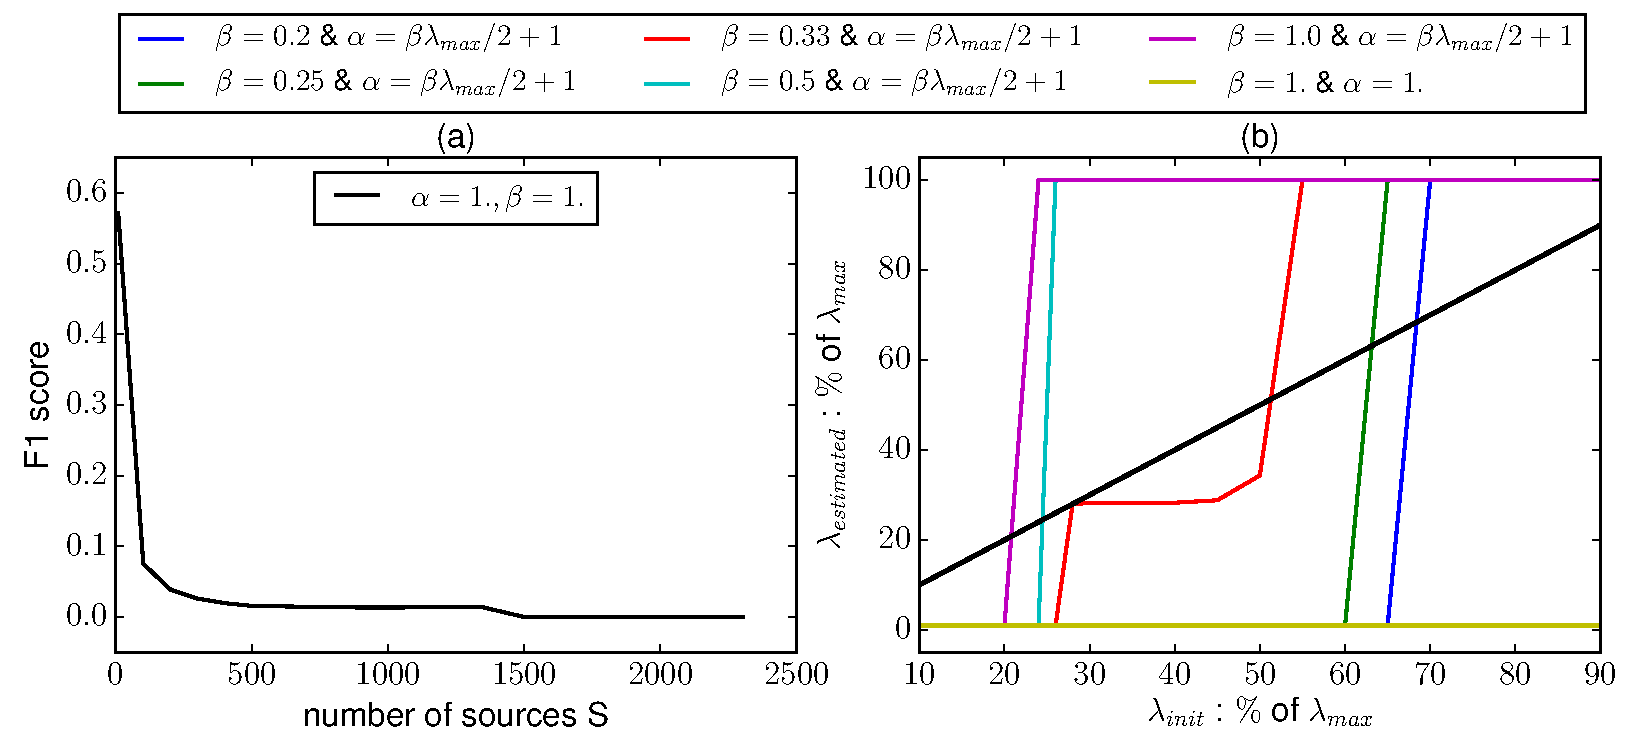
\includegraphics[width=0.95\textwidth]{hyperparam_estim/fig1_eusipco_data_size_and_fix_points_a_b}
    \caption{(a) Source identification results for different number of sources measured with F1 score
    using $\alpha=1$ and $\beta=1$. The higher the number of regressors the worse is the performance.
    (b) Estimated $\lambda$ as a function of $\lambda_{init}$ for different values of $a$ and $b$.
    The red curve for $\beta=0.33$ gives the best plateau, which demonstrates that $(a,b)$
    shall be carefully adjusted.
    }
    \label{fig:fig1}
\end{figure}

In order to illustrate the issue when using a synthesis prior for large problems, we run the estimation of the hyperparameter $\lambda$ as suggested in \cite{Figueiredo} using the $0.5$-homogeneous non-convex prior. Fig.~\ref{fig:fig1}-(a) shows the F1 score of the source reconstruction (1 for good reconstruction and 0 for bad). The source estimation is failing for almost all the range of data size. Fig.~\ref{fig:fig1}-(b) shows the results after reformulating the problem with different settings of $\alpha$ and $\beta$. One can notice that a setting as in~\cite{Figueiredo} with $\alpha=1$ and $\beta=1$ always gives an estimated $\lambda$ around $1\%$ of $\lambda_{max}$ which is not promoting the sparsity we are looking for in this kind of setting. For this aim, we varied the values of $\beta$ and computed $\alpha$ as defined before. Fig.~\ref{fig:fig1}-(b) shows that for most values of $\beta$ we have rather a too low estimation of $\lambda\approx 1\%$ or a too high $\lambda\geq 100\%$ resulting in zero source found active. Interestingly setting $\beta=1/3$ gives a plateau at $\hat{\lambda}$ close to $0.3\lambda_{max}$. This is evidence of a clear fixed point for the iterative process $\lambda^{(t+1)}=f(\lambda^{(t)})$, where $f$ is the update rule of $\lambda$ in \eqref{eq4}. We use $\beta=1/3$ from now on and its corresponding $\alpha$.

% \vspace{-7pt}
% \subsubsection{Results with one hyperparameter per source}
Fig.~\ref{fig:mxne_vs_irmxne} represents the simulated sources with stars and the estimated ones with plain lines.
% We ran the source reconstruction using both convex and non-convex penalties and compared one against several hyperparameters estimation.
Fig.~\ref{fig:mxne_vs_irmxne}-(a)-(b) display results with the $\ell_{2,1}$ and $\ell_{2,0.5}$ norms respectively, using one hyperparameter initialized to $\lambda=0.5\lambda_{max}$. One can see that in Fig.\ref{fig:mxne_vs_irmxne}-(a), the $\ell_{2,1}$ norm recovers the four sources with an amplitude bias (the estimated amplitude is lower than the exact one), and that several sources shown in light green are almost flat around zero but still found as active sources. There is no way to reduce the support without losing one of the four simulated sources,  \textit{i.e.} the $\ell_{2,1}$ norm with one hyperparameter fails to recover the exact simulated sources.
The $\ell_{2,0.5}$ norm in (b) estimates the exact four source amplitudes without amplitude bias thanks to the non-convexity\cite{irMxNE}. On the other hand, Fig.~\ref{fig:mxne_vs_irmxne}-(c) shows the results for the convex penalty using one hyperparameter per source. It can be seen that it is qualitatively equivalent to the non-convex penalty. 
The advantage of having one hyperparameter per source is to pick up only the sources involved in the measurement $\mathbf{M}$ and drop the extra almost-zero sources visible in Fig.~\ref{fig:mxne_vs_irmxne}-(a) (light green). This extension produces sparser results and less amplitude bias without casting the problem as non-convex. % MAP formulation.

\begin{figure}
	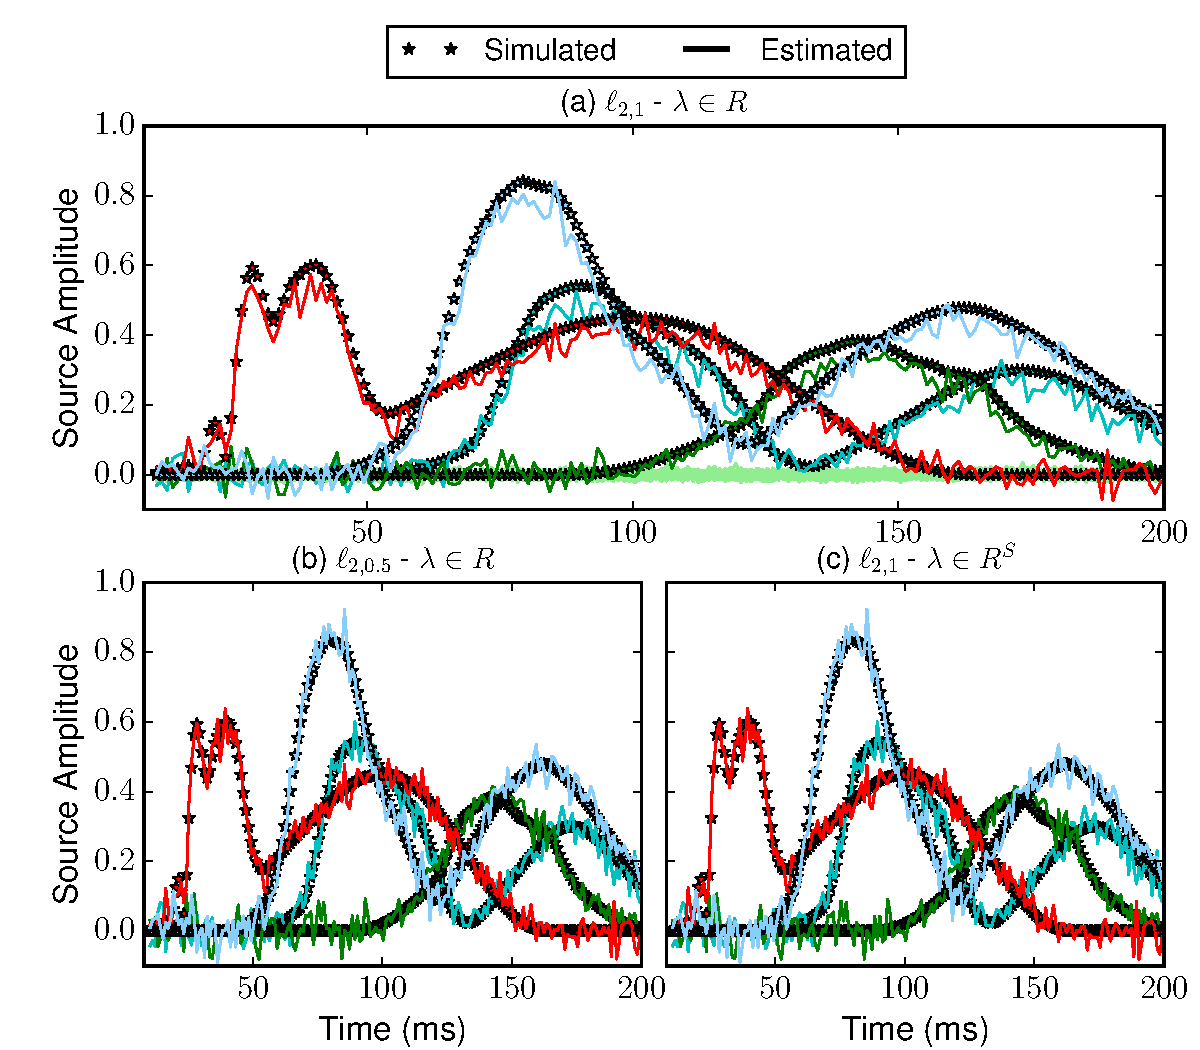
\includegraphics[width=0.95\textwidth]{hyperparam_estim/mxne_vs_irmxne}
    \caption{Source reconstruction on simulated data. (a): Source estimates obtained using $\ell_{2,1}$ with one $\lambda$. The solution is not sparse enough (the zero-sources in light green) and there is an amplitude bias between the exact amplitudes (stars) and the estimated ones (raw lines). (b): Good reconstruction of the four sources using $\ell_{2,0.5}$ and one $\lambda$, which is equivalent to the reconstruction using the $\ell_{2,1}$ norm with $\lambda\in\RR^S$ (c). Each of the four sources is encoded with a color.
    }
    %\vspace{-5pt}
    \label{fig:mxne_vs_irmxne}
\end{figure}

\subsection{Experimental results with MEG auditory data}

We applied the estimation of a single hyperparameter and a hyperparameter per source using the convex $\ell_{2,1}$ penalty on a real open dataset (MNE sample dataset \cite{MNE}). It corresponds to a dataset with $N=305$ sensors, $T=55$ time samples and $S=7498$ sources. 
Fig.~\ref{fig:sample_data} shows the source amplitudes of the two auditory sources and their positions in the brain when estimating a hyperparameter per source. When using a single hyperparameter on the convex norm $\ell_{2,1}$, multiple spurious sources are found as active which replicates the simulation on Fig.\ref{fig:mxne_vs_irmxne}-(a). These source estimates in Fig. \ref{fig:sample_data} correspond to the M100 peak (peak around 100 ms) generated in the vicinity of the bilateral auditory cortices in superior temporal gyri (the relevant auditory area).

%\subsection{Discussion and Conclusion}
%In this paper, we have explained how to address the limitations of the fixed point iteration algorithm presented in \cite{Figueiredo} when solving high-dimensional sparse synthesis problems. This required to reformulate the problem and to propose a strategy to adjust the scale parameters $\alpha$ and $\beta$ of the Gamma prior when considering
%MMV problems with group-Lasso-like penalties. Finally, we extended the approach to estimate a vector of hyperparameters. The approach was applied to the M/EEG inverse problem and then compared with the estimation of a single hyperparameter using a non-convex penalty. The results on simulated data show that using a vector of hyperparameters with the convex norm is qualitatively equivalent to the non-convex norm. This can be explained by the fact that the optimization problem for the non-convex case is solved using majorization-minimization techniques, which lead to a convex problem with some reweighting. This turns out to be similar to the multi-hyperparameter approach yet using different update rules.

\begin{figure}
%\begin{center}	
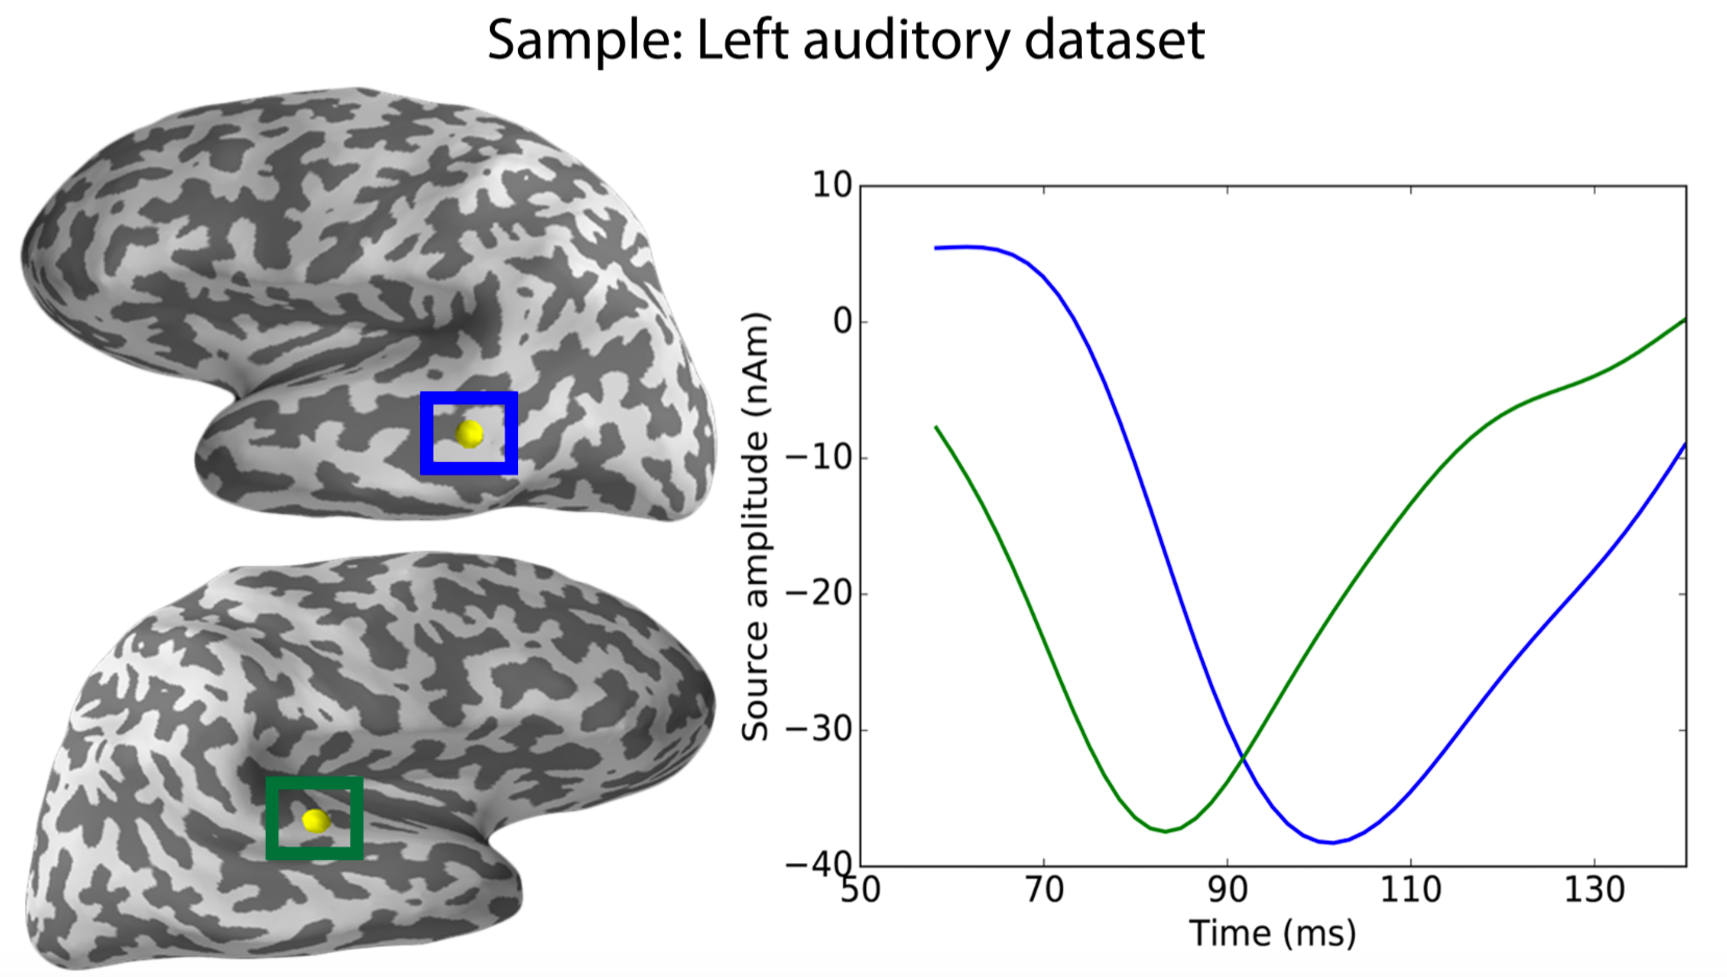
\includegraphics[width=0.95\textwidth]{hyperparam_estim/fig_sample}
    \caption{Source reconstruction on MEG auditory data (sample dataset \cite{MNE}). Source amplitude of two sources (blue and green) in the right and their corresponding positions in the brain on the left. 
    }
%\end{center}
    \label{fig:sample_data}
\end{figure}

%Concerning real data, we showed how the algorithm with a vector of hyperparameters allows us to reconstruct the two relevant sources in a MEG auditory dataset.
%Further investigations will focus on the extension of this hyperparameter estimation approach to the sparse group-Lasso $\ell_{2,1} + \ell_1$, which contains two different hyperparameters aiming to %and which is able to work with longer time windows of data by relax the temporal stationarity assumptions of simple group-Lasso-like penalties~\cite{TF-MxNE,irMxNE,bekhti2016m}.


%----------------HBM Optim------------------------------------------------------------------
\section{HBM optimization in the Bayesian formulation}
\label{sub:optimization}
%%%%%%%%%%%%%%%%%%%%%%%%%%%%%%%%%%%%%%%%%%%%%%%%%%%%%%%%%%%%%%%%%%%%%%%%%%%%%%%

The optimization problem defined in \textbf{XXX:eref}%Eq.~\eref{eq:AO-X}
 reduces to an $\ell_{2,p}$-norm regularized regression problem that can be solved as described in Section \ref{sub:MM}. For solving Eq.\textbf{XXX:eref}%~\eref{eq:AO-gamma}
 , we compute the first order optimality condition for each $i$:
\begin{eqnarray}
\label{eq:OptiGamma}
%\fl(1st)
\qquad - \frac{\fronorm{\bfX^{(k)}_{[i]}}^p}{\gamma_i^2} + \frac{1}{\beta} - \frac{( \alpha - 1 - \frac{dt}{p})}{\gamma_i} &= 0 \enspace,\label{eq:OptiGammaFirst}% \\
%\fl(2nd) \hspace{5em} \frac{2 \fronorm{\bfX^{(k+1)}_{[i]}}^p}{\gamma_i^3} + \frac{(\alpha - 1 - \frac{dt}{p})}{\gamma_i^2} &> 0 \enspace. \label{eq:OptiGammaSecond}
\end{eqnarray}
%\jo{do we need second order here? seems not so helpful, we could just say it is convex provided $\alpha \geqslant 1 + dt/p$: Less formulas, same result.}
For $\alpha \geqslant d t/p + 1$, the problem in Eq.\textbf{XXX:eref}%~\eref{eq:AO-gamma}
 is convex, and the positive root of Eq.\textbf{XXX:eref}%~\eref{eq:OptiGammaFirst}
  is given by:
\begin{equation}
\gamma_i = \beta \left( \nu + \sqrt{ \nu^2 + \frac{\fronorm{\bfX^{(k)}_{[i]}}^p}{\beta}} \right), \qquad \nu \mydef \frac{\alpha - 1 - dt/p}{2} \enspace.
\end{equation}
Note that similar rules to update the noise level were considered in the Bayesian Lasso \cite{Park_Casella08,Kyung_Gill_Ghosh_Casella10} and the Scaled Lasso (see for instance \cite{Stadler_Buhlmann_vandeGeer10,Dalalyan12}). A difference though is that the update we performed here is on the penalty term, whereas in the mentioned references, it was rather performed on the data-fitting term.


If we furthermore chose $\alpha = d t/p + 1$, then $\nu = 0$ and most terms disappear; \textbf{XXX:eref}%Eq.~\eref{eq:AO-X} and \eref{eq:AO-gamma}
 hence read:
\begin{eqnarray}
\bfX^{(k)} &= \argmin_{\bfX\in\R^{q \times t}} \left\lbrace \frac{1}{2} \fronormsq{\bfM -\bfG \bfX} + \sum_{i=1}^n  \frac{\fronorm{\bfX_{[i]}}^p}{\gamma^{(k-1)}_i} \right\rbrace \enspace, \label{eq:AO-nu0-X}\\
\gamma^{(k)}_i &= \sqrt{\beta} \sqrt{\fronorm{\bfX^{(k)}_{[i]}}^p} \, , \quad \forall i=1,\ldots,n \enspace, \label{eq:AO-nu0-gamma}
\end{eqnarray}
which can be combined to the fixed point iteration:
\begin{equation} \label{eq:AO-nu0-2}
\bfX^{(k)} = \argmin_{\bfX\in\R^{q \times t}} \left\lbrace \frac{1}{2} \fronormsq{\bfM -\bfG \bfX} + \frac{2}{\sqrt{\beta}} \sum_{i=1}^n  \frac{\fronorm{\bfX_{[i]}}^p}{2 \sqrt{\fronorm{\bfX^{(k-1)}_{[i]}}^p}} \right\rbrace \enspace .
\end{equation}
If we compare Eq.\textbf{XXX:eref}%~\eref{eq:AO-nu0-2} with Eq.~\eref{eq:MM}
 we see that we re-derived the MM algorithm for $p=1$ as an alternating optimization scheme to compute the \emph{full-MAP} estimate for a specific HBM, namely using a conditional $\ell_{2,1}$ group prior and a Gamma hyper-prior with $\alpha = dt + 1$ and $\beta = 4/\lambda^2$. Using $\bfw^{(0)}_{i} := 1$ in the MM scheme corresponds to starting with $\gamma_i^{(0)} := 1/\lambda =  2/\sqrt{\beta}$.
From previous work~\cite{strohmeier-etal:16} we know that due to the non-convexity, a good initialization of the weights $\bfw^{(0)}_{i}$ in the MM algorithm is crucial for its performance, but aside uniform initialization, only heuristic initialization strategies were used, \eg using the same re-weighting as in the sLORETA method \cite{Pa02}. In this work, we leverage the re-interpretation of the MM algorithm through the HBM framework to obtain multiple initializations in a systematic fashion, namely as samples drawn from the full posterior. This way, we can not only reach better local minima but more importantly, we can identify and characterize multiple possible sparse solutions. Such plausible solutions to the sparse regression problem in Eq.\textbf{XXX:eref}%~\eref{eq:FwdEq}
 are the modes of the posterior distribution \textbf{XXX:eref}%\eref{eq:full-post}
  with different relative probability masses.


%----------------Sampling-------------------------------------------------------------------
\section{Posterior Sampling}
\textbf{MCMC - (SC - SS) Gibbs}

\label{sub:sampling}
%%%%%%%%%%%%%%%%%%%%%%%%%%%%%%%%%%%%%%%%%%%%%%%%%%%%%%%%%%%%%%%%%%%%%%%%%%%%%%%

As outlined in Eq.\textbf{XXX:eref}%~\eref{eq:AS-X} and \eref{eq:AS-gamma}
 in Section~\ref{sub:HBM}, we sample the full posterior $\hipost$ by blocked Gibbs sampling, \ie we alternate between sampling the conditional distributions $p_{post}(\bfX|\bfM,\gamma^{(k-1)})$ and $p_{post}(\gamma|\bfM,\bfX^{(k)})$. The conditional $p_{post}(\bfX|\bfM,\gamma^{(k-1)})$ is a high dimensional distribution composed of a Gaussian likelihood and an $\ell_{2,p}$ prior, where our main interest here is $p = 1$. It was demonstrated in \cite{Lu12} that \termabb{single component Gibbs sampling}{SC Gibbs} is an efficient MCMC technique to sample such distributions. For the specific $\ell_{2,p}$ priors used here, \emph{slice sampling} can be used to perform the sub-steps in SC Gibbs sampling, namely the sampling of the one-dimensional single-component conditional densities. The resulting \emph{Slice-Within-Gibbs} sampler was examined in \cite{Lu16}. For completeness, the details of the implementation are given in \textbf{XXX:secref}%\ref{sec:DetailsGammaSampler}
 .\\
The conditional $p_{post}(\gamma|\bfM,\bfX^{(k)})$ factorizes over groups $i$:
\begin{equation}
\fl \qquad p_{post}(\gamma_i|\bfM,\bfX^{(k)}) \propto \exp \left( -\frac{\fronorm{\bfX^{(k)}_{[i]}}^p}{\gamma_i} - \frac{\gamma_i}{\beta} + (\alpha - 1 - d t/p) \log(\gamma_i) \right) \enspace. \label{eq:conPostGammai}
\end{equation}
For the case of $\alpha = d t/p + 1$, which is our main interest due to its connection to MM revealed in the previous section, Eq.\textbf{XXX:eref}%\eref{eq:conPostGammai}
 reduces to:
\begin{equation}
\fl \qquad p_{post}(\gamma_i |\bfM, \bfX^{(k)}) \propto \exp \left(- \frac{\fronorm{\bfX^{(k)}_{[i]}}^p}{\gamma_i} \right) \exp \left(- \frac{\gamma_i}{\beta} \right) \enspace, \label{eq:conPostGammaiRed}
\end{equation}
which can be sampled with a simple accept-reject algorithm as described in \textbf{XXX:secref}%\ref{sec:DetailsGammaSampler}
. The complete procedure is described in Algorithm~\ref{alg:sampling}. Therein, $K_0$ refers to the burn-in size, \ie the initial samples that are discarded, $K$ to the sample size of the blocked Gibbs sampler and $K_{SC}, K_{SS}$ to the sample sizes of the SC Gibbs and the slice sampler that carry out the sampling in the sub-steps.

{\fontsize{4}{4}\selectfont
%above is to make smaller fonts in algorithm
\begin{algorithm}[t]
\SetKwInOut{Input}{input}
\SetKwInOut{Init}{init}
\SetKwInOut{Parameter}{param}
\caption{\textsc{Block Gibbs Sampling scheme}}
\Input{$\bfM, \bfG $, $\bfX^{(-K_0)}$, $\gamma^{(-K_0)}$, $K_0$, $K$, $K_{SC}$, $K_{SS}$, $\alpha$, $\beta$}
% \Parameter{}

\For{
        $k = -K_0+1$ to $K$
    }
    {%Sample $(\bfX,\gamma) \sim p_{post}(\bfX,\gamma |\bfM)$ via \textbf{Block Gibbs:}
    Set $\bfX^{(k)} = \bfX^{(k-1)}$.\\
    \For{
    		$k_{SC} = 1$ to $K_{SC}$
    		}
    		{
    		Draw a random permutation $P$ of $\{1,\ldots,n\}$\\
    		\For{
    			$l \in P$
    			}
    			{
			Sample $\bfX_{(i,j)}^{(k)} \sim p_{post}(\bfX_{(i,j)}|\bfX_{-(i,j)}^{(k-1)},\bfM,\gamma^{(k)})$, $\forall (i,j)\in [l]$ - via $K_{SS}$ steps of \textbf{Slice Sampling} Algorithm \ref{alg:slicesampler}.
			}
		}
	{Sample $\gamma^{(k)}_{i} \sim p_{post}(\gamma_{i}|\bfM,\bfX^{(k)})$, $\forall i =1,\ldots,n$ via \textbf{Accept-Reject} Algorithm \ref{alg:acceptreject}.}

    }
\Return{$\{\bfX^{(k)},\gamma^{(k)}\}_{k=1}^K$}
\label{alg:sampling}
\end{algorithm}
}

%----------------uncertainty maps-----------------------------------------------------------
\section{Study of the different modes defining uncertainty maps of inverse problems}

%----------------Experiments-----------------------------------------------------------
\section{Experiments}

%----------------Conclusion-----------------------------------------------------------------
\section{Conclusion \& Perspective}
\label{sec:Dis}
%%%%%%%%%%%%%%%%%%%%%%%%%%%%%%%%%%%%%%%%%%%%%%%%%%%%%%%%%%%%%%%%%%%%%%%%%%%%%%%
%%%%%%%%%%%%%%%%%%%%%%%%%%%%%%%%%%%%%%%%%%%%%%%%%%%%%%%%%%%%%%%%%%%%%%%%%%%%%%%

Scientific literatures relying either on frequentist or on Bayesian statistical inference often coexist in many fields ranging from machine learning, inverse problems, signal processing or computational biology.
In this work, we started from an under-determined, ill-conditioned MMV / multi-task regression problem and examined two seemingly unrelated approaches - MM as an optimization technique for tackling non-convex optimization problems arising in frequentist regression, and HBM as a Bayesian prior modeling framework. We showed that one obtains the same algorithms, and therefore the same solutions, when considering some specific choices of models, parameters and inference strategies. In particular the parallel was done between the $\ell_{2,1/2}$-norm regularized regression by MM and the full-MAP estimation for $\ell_{2,1}$ hierarchical priors with specific Gamma hyper-priors. We further showed that this conceptual parallel can be exploited to improve the MM solution by providing well-informed algorithmic initializations.
% , and also to complement the single-point result given by MM - in our case a sparse neuronal source configuration - with a more statistical analysis of the multitude of plausible solutions to the non-convex regression problem.

% For this, we constructed a multi-layered Gibbs sampler for the joint posterior density of our HBM. This sampler has an efficient sub-sampler for $\ell_{2,1}$ priors at its core. We showed that the MCMC scheme is able to quickly jump between the different attractors of the MM scheme by using each sample as an initialization to the MM computation. Each MM computation can then be done with a state-of-the-art convex solver using block coordinate descent techniques and acceleration techniques based on active set strategies.

% As we end up in a different mode with almost every sample, this procedure is well suited to explore different plausible source configurations in more detail. \felix{we don't show this at the moment but it would be easy to add a plot.}
% \textcolor{red}{\textbf{Alternative paragraph:}

For this, we first constructed a multi-layered Gibbs sampler for the joint posterior density of our HBM.
Each sample is then used to initialize the MM step done with a state-of-the-art convex solver using block coordinate
descent techniques and acceleration strategies based on active sets. The sampler used has also an efficient sub-sampler for $\ell_{2,1}$ priors at its core. Despite the multi-modality of the posterior, the MCMC scheme is able to jump rapidely between the different attractors of the MM scheme. Indeed, using each sample as an initialization to the MM computation, one ends up in many different local minima (cf. Fig~\ref{fig:hist_real_datasets}, Fig~\ref{fig:circular_plots_LVis}). 
Therefore, this procedure allows us to reveal and explore different plausible source configurations in more details.
% }
% 

Based on this observation, we showcased how one can use the chain of local minima found by MCMC-initialized MM to analyze the variability of the different sparse solutions. Note that this is different from traditional and generic Bayesian uncertainty quantification techniques that use for example covariance estimates or credible sets derived from posterior samples~\cite{szabo2015frequentist}. It is also different from methods developed specifically for parametric M/EEG source localization based on dipole fitting~\cite{Fuchs20041442,Darvas2005355}. These latter approaches cannot easily be transferred to sparse, non-parametric approaches. Using our developed techniques on simulations and actual data, one could observe that uncertainty in M/EEG is location specific and also source configuration specific. This is of course well-known by experts in this field, but here we provide a computational approach to visualize it and quantify it.
This is an important incentive to develop such automated, data-dependent methods to quantify uncertainties in the context of M/EEG source imaging. In more conventional imaging methods such as computer tomography (CT) or magnetic resonance imaging (MRI), the signal originates from weak tissue interaction with strong external fields and the forward operator $\bfG$ depends almost exclusively on the physical properties of the scanner. In this situation, uncertainty is usually distributed in a smooth, well-known way over the image domain. Artifacts as well as real anatomical features are also easy to distinguish for a trained radiologist. The situation for M/EEG is very different. The weak signals originate from endogenous activity, and they are very dependent on dataset specific factors such as source orientation, location and attenuation which all depend on the geometry of the head of the analyzed subject. That is also why the forward matrix $\bfG$ needs to be constructed for each individual patient, after fixing the electrical properties of the head issues, which if wrong, increases the uncertainties.

When considering real data, the source to recover is often poorly understood, especially when it comes to pathological brain activity such as ictal or inter-ictal epileptic activity. In such a situation, providing a single source configuration as a result, together with an ad-hoc uncertainty quantification based on previous studies or acquired expertise, might not be an optimal use of the M/EEG data.
Instead, providing multiple hypotheses together, along with a quantification of their uncertainty, can be more useful. Indeed for applications such as pre-surgical epilepsy diagnosis, where M/EEG recordings are one of several diagnostic modalities, each candidate source configuration can provide some evidence for or against a diagnostic hypothesis that could lead to a surgery decision.
We therefore believe that extending the first steps we took here towards developing a consistent framework for interpreting and quantifying the multitude of potential results of sparse M/EEG source reconstruction approaches can have a significant impact on clinical settings.
